% !TeX program = xelatex
\documentclass[a4paper,10pt]{article}

% ============================================================================
% ១. កញ្ចប់បណ្ណាល័យ និងការកំណត់ទំព័រ (Packages & Page Setup — តាមគំរូ ls_plan.tex)
% ============================================================================
\usepackage[a4paper, left=0.95cm, right=0.95cm, top=0.85cm, bottom=0.92cm, footskip=0.52cm]{geometry}
\usepackage{amsmath}
\usepackage{unicode-math}
\usepackage{fontspec}
\usepackage{longtable, array, multirow, colortbl}
\usepackage[table]{xcolor}
\usepackage{enumitem}
\usepackage{pifont}
\usepackage{fancyhdr}
\usepackage{tikz}
\usetikzlibrary{calc, arrows.meta, decorations.pathreplacing, patterns, positioning, babel}

\makeatletter
\let\@expl@@@mark@update@singlecol@structures@@\relax
\makeatother

% --- ប្រព័ន្ធស្វែងរកទីតាំងពុម្ពអក្សរស្វ័យប្រវត្តិ (Windows Local + Cloud Repo fonts/) ---
\providecommand{\NGSFindFonts}{%
  \IfFileExists{C:/Windows/Fonts/cambria.ttc}{%
    \def\NGSSysPath{C:/Windows/Fonts/}%
    \def\NGSUserPath{C:/Users/KIT/AppData/Local/Microsoft/Windows/Fonts/}%
  }{%
    \IfFileExists{./fonts/KhmerOSsiemreap.ttf}{\def\NGSSysPath{./fonts/}\def\NGSUserPath{./fonts/}}{%
    \IfFileExists{../fonts/KhmerOSsiemreap.ttf}{\def\NGSSysPath{../fonts/}\def\NGSUserPath{../fonts/}}{%
    \IfFileExists{../../fonts/KhmerOSsiemreap.ttf}{\def\NGSSysPath{../../fonts/}\def\NGSUserPath{../../fonts/}}{%
    \IfFileExists{../../../fonts/KhmerOSsiemreap.ttf}{\def\NGSSysPath{../../../fonts/}\def\NGSUserPath{../../../fonts/}}{%
    \IfFileExists{../../../../fonts/KhmerOSsiemreap.ttf}{\def\NGSSysPath{../../../../fonts/}\def\NGSUserPath{../../../../fonts/}}{%
    \IfFileExists{../../../../../fonts/KhmerOSsiemreap.ttf}{\def\NGSSysPath{../../../../../fonts/}\def\NGSSysPath{../../../../../fonts/}}{%
    \IfFileExists{../../../../../../fonts/KhmerOSsiemreap.ttf}{\def\NGSSysPath{../../../../../../fonts/}\def\NGSUserPath{../../../../../../fonts/}}{%
      \def\NGSSysPath{../../../../../../../fonts/}\def\NGSUserPath{../../../../../../../fonts/}%
    }}}}}}}%
  }%
}
\NGSFindFonts

% ============================================================================
% ២. កំណត់ពុម្ពអក្សរ (Fonts — តាមគំរូ ls_plan.tex)
% ============================================================================
\setmathfont[Path={\NGSSysPath}, FontIndex=1, Scale=1.02]{cambria.ttc}
\defaultfontfeatures{Ligatures=TeX}

\setmainfont[
  Path={\NGSUserPath},
  Extension=.ttf,
  Script=Khmer,
  BoldFont={KhmerOSsiemreap},
  BoldFeatures={FakeBold=1.8},
  ItalicFont={KhmerOSsiemreap},
  ItalicFeatures={FakeSlant=0.25},
  BoldItalicFont={KhmerOSsiemreap},
  BoldItalicFeatures={FakeBold=1.8, FakeSlant=0.25}
]{KhmerOSsiemreap}

\newfontfamily\muol[Path={\NGSUserPath}, Extension=.ttf, Script=Khmer]{KhmerOSmuollight}
\newfontfamily\Tacteing[Path={\NGSUserPath}, Extension=.TTF]{TACTENG}
\newfontfamily\TimesEn[Path={\NGSSysPath}, Extension=.ttf, BoldFont={timesbd}, ItalicFont={timesi}, BoldItalicFont={timesbi}]{times}
\newfontfamily\CalibriFont[Path={\NGSSysPath}, Extension=.ttf]{calibri}
\newfontfamily\CourierCirc[Path={\NGSSysPath}, Extension=.ttf]{cour}

\XeTeXlinebreaklocale "km"
\XeTeXlinebreakskip = 0pt plus 1pt minus 0.1pt

% ============================================================================
% ៣. ពណ៌ និងការតុបតែង (Colors & Styles)
% ============================================================================
\definecolor{stepbg}{HTML}{D9D9D9}
\definecolor{headgray}{HTML}{E6E6E6}
\definecolor{emphred}{HTML}{C00000}

\pagestyle{fancy}
\fancyhf{}
\renewcommand{\headrulewidth}{0pt}
\fancyfoot[R]{\CalibriFont\fontsize{9pt}{11pt}\selectfont\thepage}

\setlength{\parindent}{0pt}
\setlength{\parskip}{0pt}
\setlength{\tabcolsep}{4.5pt}
\setlength{\LTpre}{2pt}
\setlength{\LTpost}{2pt}

\newcolumntype{L}[1]{>{\raggedright\arraybackslash}p{#1}}
\newcolumntype{C}[1]{>{\centering\arraybackslash}p{#1}}

% ============================================================================
% ៤. ពាក្យបញ្ជាជំនួយ (Helper Macros)
% ============================================================================
\newcommand{\en}[1]{{\TimesEn #1}}
\newcommand{\enbf}[1]{{\TimesEn\bfseries #1}}
\newcommand{\khmflourish}{{\Tacteing\fontsize{15pt}{15pt}\selectfont 3}}
\newcommand{\wcirc}{{\CourierCirc\fontsize{9.5pt}{11pt}\selectfont o}}
\newcommand{\ditem}{{\fontsize{7.5pt}{10pt}\selectfont\ding{117}}\ }
\newcommand{\fiveE}[1]{\textcolor{emphred}{\CalibriFont\bfseries #1}}
\newcommand{\redsub}[1]{\textcolor{emphred}{#1}}
\newcommand{\timenote}[1]{\textcolor{emphred}{\textit{#1}}}
\newcommand{\stepheader}[1]{\multicolumn{3}{|c|}{\cellcolor{stepbg}\muol #1} \\ \hline}
\newcommand{\cfig}[1]{{\centering\vspace{3pt}#1\vspace{3pt}\par}}
\newcommand{\cnum}[1]{\mbox{\fontsize{10.5pt}{12pt}\selectfont\ding{\numexpr181+#1\relax}}}
\newcommand{\unit}[1]{\,\text{\en{#1}}}
\newcommand{\graybox}[1]{\colorbox{headgray}{\strut #1}}

% ============================================================================
% ៥. រូបភាព TikZ ស-ខ្មៅ សម្រាប់បង្រៀនលើក្ដារខៀន និងសន្លឹកកិច្ចការ (B&W Diagrams)
% ============================================================================

% ១. E1 Engage: អន្ទាក់ពាក្យ «តូចបំផុត» លើ PPCM(6, 8)
\newcommand{\figEngageDIVTwoSix}{%
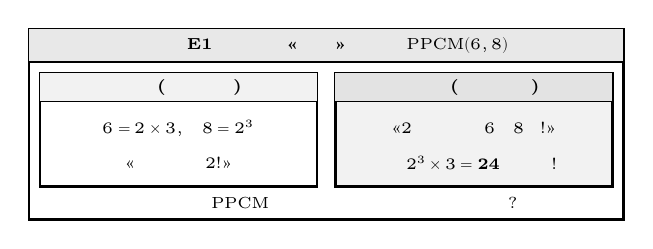
\begin{tikzpicture}[x=1cm, y=1cm, every node/.style={font=\fontsize{5.8pt}{7.7pt}\selectfont, text=black}]
  \draw[black, line width=0.9pt] (0,0) rectangle (7.55,2.42);
  \fill[gray!18] (0,2.00) rectangle (7.55,2.42);
  \draw[black, line width=0.6pt] (0,2.00) -- (7.55,2.00);
  \node at (3.775,2.21) {\textbf{បេសកកម្ម \en{E1}៖ អន្ទាក់ពាក្យ «តូចបំផុត» ក្នុងការរក $\operatorname{PPCM}(6, 8)$}};

  % Student A
  \draw[black, line width=0.8pt] (0.14,0.42) rectangle (3.66,1.86);
  \fill[gray!10] (0.14,1.50) rectangle (3.66,1.86);
  \draw[black, line width=0.5pt] (0.14,1.50) -- (3.66,1.50);
  \node at (1.90,1.68) {\textbf{សិស្ស ក (យកតែកត្តារួមតូច)}};
  \node at (1.90,1.16) {$6=2\times 3,\quad 8=2^3$};
  \node at (1.90,0.72) {«តូចបំផុតគឺយកតែ $2$!»};

  % Student B
  \draw[black, line width=0.95pt, fill=gray!10] (3.89,0.42) rectangle (7.41,1.86);
  \fill[gray!22] (3.89,1.50) rectangle (7.41,1.86);
  \draw[black, line width=0.55pt] (3.89,1.50) -- (7.41,1.50);
  \node at (5.65,1.68) {\textbf{សិស្ស ខ (ពិនិត្យពហុគុណរួម)}};
  \node at (5.65,1.16) {«$2$ ចែកមិនដាច់នឹង $6$ ឬ $8$ ទេ!»};
  \node at (5.65,0.72) {យក $2^3 \times 3 = \mathbf{24}$ ទើបចែកដាច់!};

  \node at (3.775,0.21) {\textbf{សំណួរ៖} ហេតុអ្វី $\operatorname{PPCM}$ ត្រូវយក\textbf{និទស្សន្តធំជាងគេនៃកត្តារួម គុណនឹងកត្តាមិនរួម}?};
\end{tikzpicture}}

% ២. E2 Explore: ប្រអប់ជួរឈរកត្តាបឋម ទំ.២២–២៣ សម្រាប់ PPCM(6,8) និង PPCM(18,24,36)
\newcommand{\figPrimeColsDIVTwoSix}{%
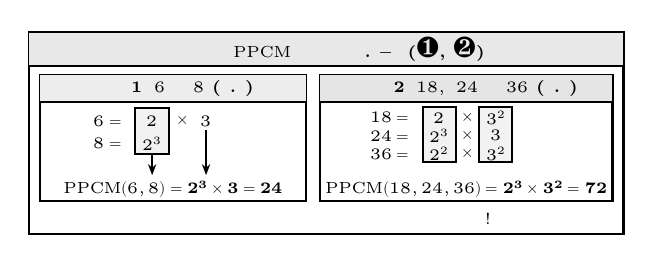
\begin{tikzpicture}[x=1cm, y=1cm, every node/.style={font=\fontsize{5.8pt}{7.6pt}\selectfont, text=black}]
  \draw[black, line width=0.9pt] (0,0) rectangle (7.55,2.56);
  \fill[gray!18] (0,2.14) rectangle (7.55,2.56);
  \draw[black, line width=0.6pt] (0,2.14) -- (7.55,2.14);
  \node at (3.775,2.35) {\textbf{ប្រអប់ជួរឈររក $\operatorname{PPCM}$ តាមសៀវភៅគោល ទំ.២២–២៣ (\cnum{1}, \cnum{2})}};

  % Left: 6 and 8 (p. 22)
  \draw[black, line width=0.8pt] (0.14,0.42) rectangle (3.52,2.02);
  \fill[gray!14] (0.14,1.68) rectangle (3.52,2.02);
  \draw[black, line width=0.5pt] (0.14,1.68) -- (3.52,1.68);
  \node at (1.83,1.85) {\textbf{ឧទាហរណ៍ 1៖ $6$ និង $8$ (ទំ.២២)}};
  \draw[black, line width=0.65pt, fill=gray!10] (1.35,1.02) rectangle (1.78,1.60);
  \node[anchor=east] at (1.30,1.44) {$6 =$};
  \node at (1.565,1.44) {$2$}; \node at (1.95,1.44) {$\times$}; \node at (2.25,1.44) {$3$};
  \node[anchor=east] at (1.30,1.15) {$8 =$};
  \node at (1.565,1.15) {$2^3$};
  \draw[-{Stealth[length=1.4mm]}, black, line width=0.55pt] (1.565,1.00) -- (1.565,0.75);
  \draw[-{Stealth[length=1.4mm]}, black, line width=0.55pt] (2.25,1.32) -- (2.25,0.75);
  \node at (1.83,0.57) {$\operatorname{PPCM}(6,8) = \mathbf{2^3 \times 3 = 24}$};

  % Right: 18, 24, 36 (p. 23)
  \draw[black, line width=0.85pt] (3.70,0.42) rectangle (7.41,2.02);
  \fill[gray!20] (3.70,1.68) rectangle (7.41,2.02);
  \draw[black, line width=0.5pt] (3.70,1.68) -- (7.41,1.68);
  \node at (5.555,1.85) {\textbf{ឧទាហរណ៍ 2៖ $18,\ 24$ និង $36$ (ទំ.២៣)}};
  \draw[black, line width=0.65pt, fill=gray!10] (5.00,0.92) rectangle (5.42,1.62);
  \draw[black, line width=0.65pt, fill=gray!10] (5.72,0.92) rectangle (6.14,1.62);
  \node[anchor=east] at (4.95,1.48) {$18 =$};
  \node at (5.21,1.48) {$2$}; \node at (5.57,1.48) {$\times$}; \node at (5.93,1.48) {$3^2$};
  \node[anchor=east] at (4.95,1.25) {$24 =$};
  \node at (5.21,1.25) {$2^3$}; \node at (5.57,1.25) {$\times$}; \node at (5.93,1.25) {$3$};
  \node[anchor=east] at (4.95,1.02) {$36 =$};
  \node at (5.21,1.02) {$2^2$}; \node at (5.57,1.02) {$\times$}; \node at (5.93,1.02) {$3^2$};
  \node at (5.555,0.57) {$\operatorname{PPCM}(18,24,36) = \mathbf{2^3 \times 3^2 = 72}$};

  \node at (3.775,0.20) {គោលការណ៍៖ ទម្លាក់\textbf{និទស្សន្តធំជាងគេនៃកត្តារួម} គុណជាមួយនឹង\textbf{គ្រប់កត្តាមិនរួម}!};
\end{tikzpicture}}

% ៣. E4 Elaborate: លំហាត់គំរូ ទំ.២៣ (រៀបប័ណ្ណ 12cm x 9cm ជាការេតូចបំផុត 36cm)
\newcommand{\figCardsDIVTwoSix}{%
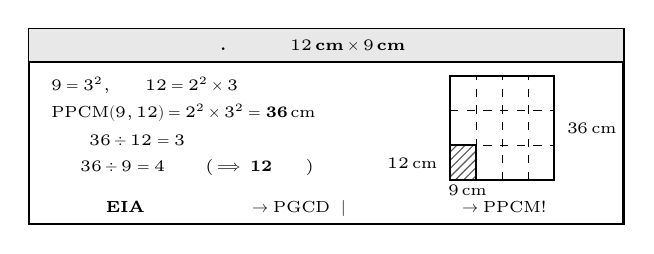
\begin{tikzpicture}[x=1cm, y=1cm, every node/.style={font=\fontsize{5.8pt}{7.6pt}\selectfont, text=black}]
  \draw[black, line width=0.9pt] (0,0) rectangle (7.55,2.48);
  \fill[gray!18] (0,2.06) rectangle (7.55,2.48);
  \draw[black, line width=0.6pt] (0,2.06) -- (7.55,2.06);
  \node at (3.775,2.27) {\textbf{លំហាត់គំរូ ទំ.២៣៖ រៀបប័ណ្ណ $12\unit{cm}\times 9\unit{cm}$ បង្កើតការេតូចបំផុត}};

  % Left calculation
  \node[anchor=west] at (0.16,1.76) {$9 = 3^2,\qquad 12 = 2^2 \times 3$};
  \node[anchor=west] at (0.16,1.42) {$\operatorname{PPCM}(9,12) = 2^2\times 3^2 = \mathbf{36\unit{cm}}$};
  \node[anchor=west] at (0.16,1.06) {បណ្ដោយ៖ $36\div 12 = 3$ សន្លឹក};
  \node[anchor=west] at (0.16,0.72) {ទទឹង៖ $36\div 9 = 4$ សន្លឹក ($\implies \mathbf{12}$ សន្លឹក)};

  % Right square matching textbook p.23 (3 cols of width 0.56, 4 rows of height 0.33 -> 1.68 x 1.32 visual or true square 1.32 x 1.32!)
  % True square 1.32 x 1.32 divided into 4 columns of 9cm (width 0.33) and 3 rows of 12cm (height 0.44) — matching textbook p.23 vertical 12cm x horizontal 9cm card!
  \begin{scope}[shift={(5.35,0.56)}]
    \fill[pattern=north east lines, pattern color=black!65] (0,0) rectangle (0.33,0.44);
    \draw[black, line width=0.8pt] (0,0) rectangle (1.32,1.32);
    \foreach \i in {1,2,3} {\draw[black, dashed, line width=0.4pt] (\i*0.33,0) -- (\i*0.33,1.32);}
    \foreach \j in {1,2} {\draw[black, dashed, line width=0.4pt] (0,\j*0.44) -- (1.32,\j*0.44);}
    \draw[black, line width=0.7pt] (0,0) rectangle (0.33,0.44);
    \node[anchor=east] at (-0.04,0.22) {$12\unit{cm}$};
    \node at (0.22,-0.13) {$9\unit{cm}$};
    \node[anchor=west] at (1.36,0.66) {$36\unit{cm}$};
  \end{scope}

  \node at (3.775,0.20) {\textbf{\en{EIA}៖} បំបែកចតុកោណកែងជាការេ $\to \operatorname{PGCD}$ $\;\mid\;$ ផ្គុំប័ណ្ណតូចៗជាការេធំ $\to \operatorname{PPCM}$!};
\end{tikzpicture}}

% ៣ខ. E5 Practice: ប្រតិបត្តិសំយោគ ទំ.២៣ (58, 73, 85 ចែកនឹង x សល់ 2, 3, 1 -> x = 14)
\newcommand{\figPracticeDIVTwoSix}{%
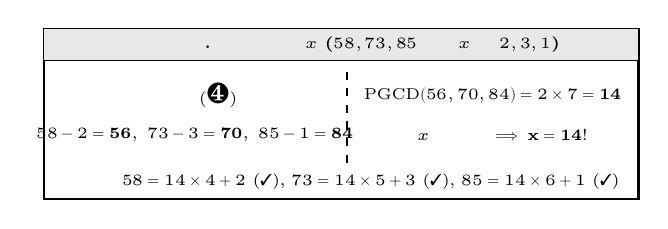
\begin{tikzpicture}[x=1cm, y=1cm, every node/.style={font=\fontsize{5.7pt}{7.5pt}\selectfont, text=black}]
  \draw[black, line width=0.9pt] (0,0) rectangle (7.55,2.16);
  \fill[gray!18] (0,1.76) rectangle (7.55,2.16);
  \draw[black, line width=0.6pt] (0,1.76) -- (7.55,1.76);
  \node at (3.775,1.96) {\textbf{ប្រតិបត្តិសំយោគ ទំ.២៣៖ រកចំនួនពីរខ្ទង់ $x$ ($58, 73, 85$ ចែកនឹង $x$ សល់ $2, 3, 1$)}};
  \node at (1.92,1.32) {ដកសំណល់ចេញ (\cnum{4})៖};
  \node at (1.92,0.82) {$58-2=\mathbf{56},\ 73-3=\mathbf{70},\ 85-1=\mathbf{84}$};
  \draw[black, dashed, line width=0.5pt] (3.85,0.46) -- (3.85,1.66);
  \node at (5.70,1.32) {$\operatorname{PGCD}(56, 70, 84) = 2\times 7 = \mathbf{14}$};
  \node at (5.70,0.82) {ដោយ $x$ មានពីរខ្ទង់ $\implies \mathbf{x = 14}$!};
  \node at (3.775,0.22) {ផ្ទៀងផ្ទាត់៖ $58=14\times 4+2$ (\ding{51}),\ $73=14\times 5+3$ (\ding{51}),\ $85=14\times 6+1$ (\ding{51})};
\end{tikzpicture}}

% ៤. E5 Evaluate: សំណួរវិនិច្ឆ័យ A-D លើ A = 2^3 x 3 និង B = 2 x 3^2 x 5
\newcommand{\figExitDIVTwoSix}{%
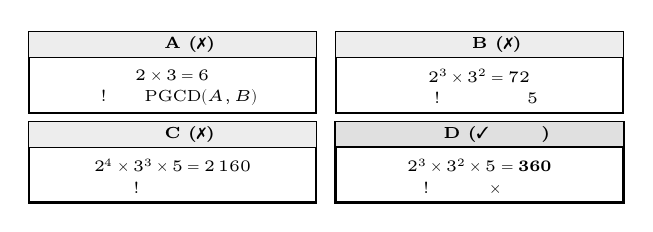
\begin{tikzpicture}[x=1cm, y=1cm, every node/.style={font=\fontsize{5.8pt}{7.5pt}\selectfont, text=black}]
  % Choice A
  \draw[black, line width=0.8pt] (0,1.14) rectangle (3.65,2.16);
  \fill[gray!14] (0,1.84) rectangle (3.65,2.16);
  \draw[black, line width=0.5pt] (0,1.84) -- (3.65,1.84);
  \node at (1.825,2.00) {\textbf{ជម្រើស \en{A} (\ding{55})}};
  \node at (1.825,1.61) {$2 \times 3 = 6$};
  \node at (1.825,1.33) {ខុស! នេះជា $\operatorname{PGCD}(A,B)$};

  % Choice B
  \draw[black, line width=0.8pt] (3.90,1.14) rectangle (7.55,2.16);
  \fill[gray!14] (3.90,1.84) rectangle (7.55,2.16);
  \draw[black, line width=0.5pt] (3.90,1.84) -- (7.55,1.84);
  \node at (5.725,2.00) {\textbf{ជម្រើស \en{B} (\ding{55})}};
  \node at (5.725,1.61) {$2^3 \times 3^2 = 72$};
  \node at (5.725,1.33) {ខុស! ភ្លេចកត្តាមិនរួម $5$};

  % Choice C
  \draw[black, line width=0.8pt] (0,0) rectangle (3.65,1.02);
  \fill[gray!14] (0,0.70) rectangle (3.65,1.02);
  \draw[black, line width=0.5pt] (0,0.70) -- (3.65,0.70);
  \node at (1.825,0.86) {\textbf{ជម្រើស \en{C} (\ding{55})}};
  \node at (1.825,0.47) {$2^4 \times 3^3 \times 5 = 2\,160$};
  \node at (1.825,0.19) {ខុស! ច្រឡំបូកនិទស្សន្ត};

  % Choice D (Correct)
  \draw[black, line width=1.05pt] (3.90,0) rectangle (7.55,1.02);
  \fill[gray!24] (3.90,0.70) rectangle (7.55,1.02);
  \draw[black, line width=0.6pt] (3.90,0.70) -- (7.55,0.70);
  \node at (5.725,0.86) {\textbf{ជម្រើស \en{D} (\ding{51} ត្រឹមត្រូវ)}};
  \node at (5.725,0.47) {$2^3 \times 3^2 \times 5 = \mathbf{360}$};
  \node at (5.725,0.19) {ត្រូវ! កត្តារួមធំ $\times$ កត្តាមិនរួម};
\end{tikzpicture}}

\begin{document}
\fontsize{10pt}{15.2pt}\selectfont

% ============================================================================
% ក្បាលរដ្ឋបាល (Administrative Header — តាមគំរូ ls_plan.tex)
% ============================================================================
{\centering
  {\muol\fontsize{11pt}{16pt}\selectfont ព្រះរាជាណាចក្រកម្ពុជា\par}
  {\muol\fontsize{11pt}{16pt}\selectfont ជាតិ សាសនា ព្រះមហាក្សត្រ\par}
  \vspace{-3pt}{\khmflourish\par}
}

\vspace{1pt}
{\muol\fontsize{10pt}{15.5pt}\selectfont
មន្ទីរអប់រំ យុវជន និងកីឡា ខេត្តកំពង់ធំ\par
ការិយាល័យអប់រំ យុវជន និងកីឡា ស្រុកកំពង់ស្វាយ\par
អនុវិទ្យាល័យព្រះក្រសាំង\par}

\vspace{2pt}
{\centering{\muol\fontsize{11.5pt}{17pt}\selectfont កិច្ចតែងការបង្រៀន\par}}
\vspace{2pt}

% --- ព័ត៌មានទូទៅ ---
{\hspace*{2.8cm}\renewcommand{\arraystretch}{1.08}
\begin{tabular}{@{}l@{\hspace{0.35cm}}p{2.9cm}@{\hspace{0.15cm}}c@{\hspace{0.25cm}}l@{}}
  - & មុខវិជ្ជា & : & គណិតវិទ្យា ថ្នាក់ទី៧ (ពីជគណិត) \\
  - & ចំណងជើងមេរៀន & : & មេរៀនទី២៖ តួចែកនិងពហុគុណ \\
  - & ចំណងជើងរង & : & ៦. ពហុគុណរួមតូចបំផុត (\en{PPCM}) និងសំយោគមេរៀនទី២ (ទំ.២២--២៣) \\
  - & រយៈពេល & : & ១ ម៉ោងសិក្សា (៥០ នាទី) \\
  - & បង្រៀនដោយ & : & ហុក ប៊ុនថែន \\
  - & កាលបរិច្ឆេទ & : & ថ្ងៃពុធ ទី១៨ ខែវិច្ឆិកា ឆ្នាំ២០២៦ \\
\end{tabular}\par}

\vspace{2pt}

% --- I. វត្ថុបំណង ---
{\muol\fontsize{10pt}{15.5pt}\selectfont \enbf{I.} វត្ថុបំណង\par}
\vspace{1pt}
{\renewcommand{\arraystretch}{1.10}
\begin{tabular}{@{}p{0.55cm}@{}p{2.35cm}@{\hspace{0.15cm}}c@{\hspace{0.25cm}}p{14.95cm}@{}}
  \hfill\wcirc\hspace{0.2cm} & វិជ្ជាសម្បទា & : & សិស្សប្រាប់បានពីនិយមន័យនិងវិធានរកពហុគុណរួមតូចបំផុត (\en{PPCM}) ព្រមទាំងលក្ខណៈខុសគ្នារវាង \en{PGCD} និង \en{PPCM} បានត្រឹមត្រូវ (ទំ.២២--២៣) ។ \\
  \hfill\wcirc\hspace{0.2cm} & បំណិនសម្បទា & : & សិស្សគណនា \en{PPCM} តាមផលគុណកត្តាបឋម និងជ្រើសរើស \en{PGCD} ឬ \en{PPCM} ដោះស្រាយចំណោទសំយោគលើសន្លឹកកិច្ចការបានត្រឹមត្រូវ ។ \\
  \hfill\wcirc\hspace{0.2cm} & ចរិយាសម្បទា & : & សិស្សមានទម្លាប់វិភាគអត្ថន័យចំណោទមុនជ្រើសរូបមន្ត មិនច្រឡំក្បួន \en{PGCD/PPCM} និងសហការដោះស្រាយបញ្ហាក្នុងក្រុមដោយសកម្ម ។ \\
\end{tabular}\par}

\vspace{2pt}

% --- II. សម្ភារៈឧបទេស ---
{\muol\fontsize{10pt}{15.5pt}\selectfont \enbf{II.} សម្ភារៈឧបទេស\par}
\vspace{1pt}
\hspace*{0.55cm}$\bullet$\ សៀវភៅសិក្សាគោលថ្នាក់ទី៧ (ទំ.២២--២៤) ក្ដារខៀន ដីស/ហ្វឺត និង\textbf{សន្លឹកកិច្ចការសិស្សបំពេញចន្លោះ ស-ខ្មៅ} (កូដ \en{DIV26} ទំព័រ ១--២ សម្រាប់សិស្ស និងទំព័រ ៣ ប្លង់ក្ដារខៀន/ចម្លើយគ្រូ — គ្មានប្រើ \en{LCD})\par

\vspace{2pt}

% --- III. វិធីសាស្រ្តបង្រៀន ---
{\muol\fontsize{10pt}{15.5pt}\selectfont \enbf{III.} វិធីសាស្រ្តបង្រៀន\par}
\vspace{1pt}
{\renewcommand{\arraystretch}{1.08}
\begin{tabular}{@{}p{0.55cm}@{}p{2.35cm}@{\hspace{0.15cm}}c@{\hspace{0.25cm}}p{14.95cm}@{}}
  \hfill$\bullet$\hspace{0.2cm} & គោលវិធី & : & សិស្សមជ្ឈមណ្ឌល (សន្លឹកកិច្ចការបំពេញចន្លោះជាគោល + ការពិភាក្សាជាក្រុមតូច ៣ នាក់) \\
  \hfill$\bullet$\hspace{0.2cm} & យុទ្ធវិធីបង្រៀន & : & គំរូស្ថាបនានិយម \en{5Es} រួមបញ្ចូល \textbf{តារាងញែកលក្ខណៈឆ្លាស់គ្នា \en{PGCD} ទល់នឹង \en{PPCM} (\en{Contrastive Discrimination})} \\
\end{tabular}\par}

\vspace{2pt}

% --- IV. ដំណើរការបង្រៀន ---
{\muol\fontsize{10pt}{15.5pt}\selectfont \enbf{IV.} ដំណើរការបង្រៀន\par}

{\renewcommand{\arraystretch}{1.14}
\begin{longtable}{|L{5.50cm}|L{7.90cm}|L{4.80cm}|}
\hline
\multicolumn{1}{|c|}{\cellcolor{headgray}\muol សកម្មភាពគ្រូ} &
\multicolumn{1}{c|}{\cellcolor{headgray}\muol ខ្លឹមសារមេរៀន} &
\multicolumn{1}{c|}{\cellcolor{headgray}\muol សកម្មភាពសិស្ស} \\
\hline
\endfirsthead

\hline
\multicolumn{1}{|c|}{\cellcolor{headgray}\muol សកម្មភាពគ្រូ} &
\multicolumn{1}{c|}{\cellcolor{headgray}\muol ខ្លឹមសារមេរៀន} &
\multicolumn{1}{c|}{\cellcolor{headgray}\muol សកម្មភាពសិស្ស} \\
\hline
\endhead

% ==================== ជំហានទី១ (2min) ====================
\stepheader{ជំហានទី១ \enbf{(}រដ្ឋបាលថ្នាក់\enbf{)}}
$\bullet$ ពិនិត្យវត្តមាន អនាម័យ និងសណ្ដាប់ធ្នាប់ថ្នាក់រៀន \par
$\bullet$ រៀបចំក្រុមតូច ៣ នាក់តាមតុ និងចែក\textbf{សន្លឹកកិច្ចការសិស្ស (\en{DIV26} ទំព័រ ១–២)}
&
$\bullet$ រដ្ឋបាលថ្នាក់ អនាម័យ និងវិន័យសិក្សា \par
$\bullet$ ចែកសន្លឹកកិច្ចការម្នាក់ ១ សន្លឹក សម្រាប់បំពេញតាមដំណាក់កាល \en{E1--E5}
&
$\circ$ ប្រធានថ្នាក់រាយការណ៍វត្តមានសិស្ស \par
$\circ$ ទទួលសន្លឹកកិច្ចការ សរសេរឈ្មោះ និងអង្គុយតាមក្រុម ៣ នាក់ \\
\hline

% ==================== ជំហានទី២ (9min: កំណែ <=3m + រំលឹក 3m + E1 3m) ====================
\stepheader{ជំហានទី២ \enbf{(}កិច្ចការផ្ទះ \enbf{+} ទំនាក់ទំនងមេរៀនថ្មី\enbf{)}}
\ditem \textbf{កំណែកិច្ចការផ្ទះ ($\le\text{\enbf{3\,min}}$)} \par
$\bullet$ ហៅសិស្សផ្ទៀងផ្ទាត់ចម្លើយលំហាត់ទំ.២៤ លេខ ៦, ៨, ១០ លើក្ដារខៀនឆ្វេង
&
{\centering\redsub{កំណែកិច្ចការផ្ទះមេរៀនមុន (ទំ.២៤ លេខ ៦, ៨, ១០)}\par}
$\bullet$ \textbf{លេខ ៦៖} ក. $3$, ខ. $2$, គ. $4$, ឃ. $32$, ង. $12$, ច. $12$ \par
$\bullet$ \textbf{លេខ ៨៖} $x=12a, y=12b$ ($a+b=6,\ \operatorname{PGCD}(a,b)=1$) $\implies \mathbf{x=12, y=60}$ \par
$\bullet$ \textbf{លេខ ១០៖} ជ្រុងកូនកន្សែងដៃការេធំបំផុត៖ $\operatorname{PGCD}(24,56) = \mathbf{8\unit{cm}}$
&
$\circ$ ផ្ទៀងចម្លើយលេខ ៦, ៨, ១០ និងកែចូលសៀវភៅ \\[3pt]

\ditem \textbf{រំលឹកមេរៀនទាក់ទង (\enbf{3min})} \par
$\bullet$ សួរ៖ «ចូររាយពហុគុណមិនសូន្យ ៥ តួដំបូងនៃ $6$ និងនៃ $8$ រួចបំបែក $6, 8$ ជាកត្តាបឋម!»
&
{\centering\redsub{រំលឹកពហុគុណមិនសូន្យ និងកត្តាបឋម}\par}
$\bullet$ ពហុគុណនៃ $6$: $6, 12, 18, 24, 30, \dots$ \quad នៃ $8$: $8, 16, 24, 32, 40, \dots$ \par
$\bullet$ បំបែក៖ $6 = \mathbf{2 \times 3}$ \quad និង \quad $8 = \mathbf{2^3}$
&
$\circ$ រាយពហុគុណនៃ $6, 8$ និងបំបែក $6=2\times 3,\ 8=2^3$ \\[3pt]

\fiveE{E1 - Engage (3min)} \timenote{(កុំទាន់ផ្ដល់ចម្លើយ)} \par
\ditem \textbf{បេសកកម្មអន្ទាក់ពាក្យ «តូចបំផុត» ក្នុង $\operatorname{PPCM}(6, 8)$ (\en{E1})}
&
\redsub{បេសកកម្ម \en{E1}៖ តើអ្នកណារកពហុគុណរួមតូចបំផុតនៃ $6$ និង $8$ ត្រូវ?}
&
$\circ$ អានស្ថានភាពបញ្ហា \en{E1} \\[3pt]

$\bullet$ ឱ្យសិស្សពិភាក្សាជាគូលើសន្លឹកកិច្ចការ \en{E1} រវាងសិស្ស ក ($2$) និងសិស្ស ខ ($24$)
&
$\bullet$ \textbf{សិស្ស ក៖} «ព្រោះរកពហុគុណរួម\textbf{តូចបំផុត} ត្រូវយកតែកត្តារួមតូច គឺ $2$!» \par
$\bullet$ \textbf{សិស្ស ខ៖} «$2$ ចែកមិនដាច់នឹង $6$ ឬ $8$ ទេ! ត្រូវយក $2^3\times 3 = 24$ ទើបចែកដាច់ទាំងពីរ!»
&
$\circ$ ពិភាក្សាជាគូ និងគូស \ding{51} ក្នុងប្រអប់ \en{E1} \\[3pt]

&
\cfig{\figEngageDIVTwoSix}
& \\
\hline

% ==================== ជំហានទី៣ (17min: E2 11m + E3 6m) ====================
\stepheader{ជំហានទី៣ \enbf{(}ខ្លឹមសារមេរៀនថ្មី\enbf{)}}
\fiveE{E2 - Explore (11min)} \par
$\bullet$ សរសេរចំណងជើងរង \textbf{៦. ពហុគុណរួមតូចបំផុត (\en{PPCM} ឬ \en{LCM})} \par
\ditem \textbf{សកម្មភាព ១៖ ប្រៀបធៀប ២ វិធីលើ $6$ និង $8$ (ឧទាហរណ៍ 1 ទំ.២២, \enbf{5.5min})}
&
៦. ពហុគុណរួមតូចបំផុត (\en{PPCM} ឬ \en{LCM}) (ទំ.២២--២៣) \par
$\bullet$ \textbf{ឧទាហរណ៍ 1 (រក $\operatorname{PPCM}$ នៃ $6$ និង $8$)៖} \par
\hspace*{0.15cm}-- \textbf{វិធីទី 1 (រាយពហុគុណ)៖} ពហុគុណរួមនៃ $6$ និង $8$ គឺ $24, 48, \dots \implies \operatorname{PPCM}(6,8) = \mathbf{24}$
&
$\circ$ រកពហុគុណរួមលើបញ្ជី ឃើញតូចបំផុតគឺ $24$ លើ \en{E2-A} \\[3pt]

$\bullet$ ឱ្យសិស្សតម្រឹមជួរឈរកត្តាបឋមនៃ $6$ និង $8$ លើ \en{E2-A} តាមសៀវភៅគោល ទំ.២២
&
\hspace*{0.15cm}-- \textbf{វិធីទី 2 (កត្តាបឋម)៖} $6 = 2 \times 3$ និង $8 = 2^3$ \par
ទម្លាក់កត្តារួមនិទស្សន្តធំ ($2^3$) គុណនឹងកត្តាមិនរួម ($3$)៖ $\operatorname{PPCM}(6,8) = 2^3\times 3 = \mathbf{24}$
&
$\circ$ ទម្លាក់ $2^3$ និង $3$ គុណគ្នាបាន $24$ ដូចគ្នា! \\[3pt]

\ditem \textbf{សកម្មភាព ២៖ ចំនួនបីតួ និងប្រៀបធៀបនឹង $\operatorname{PGCD}$ (ឧទាហរណ៍ 2 ទំ.២២–២៣, \enbf{5.5min})} \par
$\bullet$ ឱ្យសិស្សរក $\operatorname{PPCM}(18, 24, 36)$ និងប្រៀបធៀបនឹង $\operatorname{PGCD}(18, 24, 36)$ លើ \en{E2-B}
&
$\bullet$ \textbf{ឧទាហរណ៍ 2៖} $18 = 2\times 3^2$, $24 = 2^3\times 3$, $36 = 2^2\times 3^2$ \par
$\implies \operatorname{PPCM}(18, 24, 36) = 2^3 \times 3^2 = 8\times 9 = \mathbf{72}$ \par
(ប្រៀបធៀប៖ ឯ $\operatorname{PGCD}(18, 24, 36) = 2 \times 3 = \mathbf{6}$!)
&
$\circ$ បំពេញប្រអប់ជួរឈររកឃើញ $\operatorname{PPCM}=72$ ទល់នឹង $\operatorname{PGCD}=6$ \\[3pt]

&
\cfig{\figPrimeColsDIVTwoSix}
& \\[3pt]

% --- E3 Explain (6min) ---
\fiveE{E3 - Explain (6min)} \par
$\bullet$ ដឹកនាំសិស្សសង្ខេបប្រអប់ «ជាទូទៅ» (ទំ.២៣) លើសន្លឹកកិច្ចការ \en{E3}
&
$\bullet$ \textbf{ជាទូទៅ (ទំ.២៣)៖} ដើម្បីរក $\operatorname{PPCM}$ នៃពីរ ឬច្រើនចំនួន គេបំបែកចំនួននីមួយៗជាផលគុណកត្តាបឋម រួចគុណ\graybox{កត្តារួមដែលមាននិទស្សន្តធំជាងគេ} ជាមួយនឹង\graybox{កត្តាមិនរួម} ។
&
$\circ$ បំពេញប្រអប់វិធានទូទៅលើ \en{E3} \\[3pt]

$\bullet$ សង្ខេប\textbf{ទំនាក់ទំនងពិសេស} សម្រាប់ពីរចំនួន $a$ និង $b$
&
$\bullet$ \textbf{ទំនាក់ទំនងពិសេស៖} ចំពោះពីរចំនួន $a, b$ គេមាន $\operatorname{PGCD}(a,b)\times\operatorname{PPCM}(a,b) = a\times b$ (ហើយបើ $a, b$ បឋមរវាងគ្នា នោះ $\operatorname{PPCM}(a,b) = a\times b$) ។
&
$\circ$ ផ្ទៀងផ្ទាត់ $6\times 8 = 2\times 24 = 48$ \\[3pt]

$\bullet$ ភ្ជាប់\textbf{ធនាគារហេតុផល \cnum{1}--\cnum{2}} លើក្ដារខៀន និងសន្លឹកកិច្ចការ
&
\textbf{ធនាគារហេតុផល (\en{Warrant Bank})៖} \par
\cnum{1} \textbf{លក្ខខណ្ឌពហុគុណរួម៖} $\operatorname{PPCM}(a,b)$ ចែកដាច់នឹងទាំង $a$ និង $b$ ($\operatorname{PPCM} \ge \max(a,b)$) \par
\cnum{2} \textbf{ក្បួនកត្តាបឋម $\operatorname{PPCM}$៖} កត្តារួម (និទស្សន្តធំជាងគេ) $\times$ គ្រប់កត្តាមិនរួមទាំងអស់
&
$\circ$ ផ្ទៀងលេខកូដ \cnum{1}--\cnum{2} លើសន្លឹកកិច្ចការ \\[3pt]

$\bullet$ ភ្ជាប់\textbf{ធនាគារហេតុផល \cnum{3}--\cnum{4}} សម្រាប់ញែកប្រភេទចំណោទសំយោគ
&
\cnum{3} \textbf{ញែកចំណោទ៖} កាត់បំបែក/ចែកស្មើ $\to \operatorname{PGCD}$ $\;\mid\;$ រៀបផ្គុំ/ជួបដំណាលគ្នា $\to \operatorname{PPCM}$ \par
\cnum{4} \textbf{ចំណោទសំណល់៖} បើ $N$ ចែកនឹង $x$ សល់ $r$ នោះ $(N - r)$ ចែកដាច់នឹង $x$ (ដែល $x > r$)
&
$\circ$ ផ្ទៀងលេខកូដ \cnum{3}--\cnum{4} សម្រាប់ដោះស្រាយចំណោទសំយោគ \\
\hline

% ==================== ជំហានទី៤ (20min: E4 10m + E5 10m) ====================
\stepheader{ជំហានទី៤ \enbf{(}ពង្រីកចំណេះដឹង\enbf{)}}
\fiveE{E4 - Elaborate (10min)} \par
\ditem \textbf{លំហាត់គំរូតាមសៀវភៅគោល ទំ.២៣ (រៀបប័ណ្ណ $12\unit{cm}\times 9\unit{cm}$ ជាការេតូចបំផុត)}
&
{\muol លំហាត់គំរូ} \textbf{(សៀវភៅគោល ទំ.២៣ — រៀបប័ណ្ណចតុកោណកែងបង្កើតការេ)៖} \par
$\bullet$ រៀបសន្លឹកប័ណ្ណតូចៗបណ្ដោយ $12\unit{cm}$ និងទទឹង $9\unit{cm}$ តាមទិសដៅដូចគ្នាបង្កើតបានការេតូចបំផុត ។
&
$\circ$ អានប្រធានលំហាត់គំរូ និងកត់សម្គាល់ទំហំប័ណ្ណ $12\unit{cm}\times 9\unit{cm}$ \\[3pt]

$\bullet$ ដឹកនាំសិស្សបកស្រាយហេតុផលប្រើ $\operatorname{PPCM}$ និងគណនាជ្រុងការេលើ \en{E4}
&
$\bullet$ \textbf{១) ប្រវែងជ្រុងការេតូចបំផុត៖} ជ្រុងការេត្រូវជាពហុគុណរួមតូចបំផុតនៃ $9$ និង $12$ (\cnum{3})៖ \par
ដោយ $9 = 3^2$ និង $12 = 2^2\times 3 \implies \operatorname{PPCM}(9,12) = 2^2\times 3^2 = \graybox{$36\unit{cm}$}$ (\cnum{2})
&
$\circ$ បំបែក $9, 12$ និងគណនាឃើញជ្រុងការេ $36\unit{cm}$ \\[3pt]

$\bullet$ ឱ្យសិស្សគណនាចំនួនសន្លឹកប័ណ្ណដែលត្រូវប្រើដើម្បីរៀបបានការេនោះ
&
$\bullet$ \textbf{២) ចំនួនប័ណ្ណត្រូវប្រើ៖} $(36\div 12)\times(36\div 9) = 3\times 4 = \graybox{$12$ សន្លឹក}$ ។
&
$\circ$ គណនាឃើញត្រូវប្រើប័ណ្ណ $3\times 4 = 12$ សន្លឹក \\[3pt]

&
\cfig{\figCardsDIVTwoSix}
& \\[3pt]

$\bullet$ សួរសំណួរឆ្លុះបញ្ចាំង \textbf{\en{EIA Looking-Back} (1min)} ប្រៀបធៀបការ៉ូបន្ទប់ទឹក ទល់នឹង ប័ណ្ណការេ
&
\textbf{\en{EIA Looking-Back}៖} «ហេតុអ្វីក្រាលការ៉ូបន្ទប់ទឹក $90\times 126$ ប្រើ $\operatorname{PGCD}$ ឯរៀបប័ណ្ណ $12\times 9$ ប្រើ $\operatorname{PPCM}$?» ($\to$ ក្រាលការ៉ូគឺ\textbf{បំបែក}ចតុកោណកែងធំជាការេតូចៗ ឯរៀបប័ណ្ណគឺ\textbf{ផ្គុំ}ចតុកោណកែងតូចៗជាការេធំ!)
&
$\circ$ ញែកដាច់រវាងការបំបែក ($\operatorname{PGCD}$) និងការផ្គុំ ($\operatorname{PPCM}$) \\[3pt]

% --- E5 Evaluate (10min) ---
\fiveE{E5 - Evaluate (10min)} \par
\ditem \textbf{ប្រតិបត្តិសំយោគមេរៀនទី២ ជាក្រុមតូច ៣ នាក់ (4min, សន្លឹកកិច្ចការ \en{E5})} \par
$\bullet$ ឱ្យក្រុមសិស្សដោះស្រាយប្រតិបត្តិទំ.២៣៖ រកចំនួនពីរខ្ទង់ $x$ ($58, 73, 85$ ចែកនឹង $x$ សល់ $2, 3, 1$)
&
{\muol លំហាត់ប្រតិបត្តិ} \textbf{(សៀវភៅគោល ទំ.២៣ — សំយោគមេរៀនទី២)៖} \par
$\bullet$ ដកសំណល់ចេញ (\cnum{4})៖ $58-2=56,\ 73-3=70,\ 85-1=84$ សុទ្ធតែចែកដាច់នឹង $x$ \par
$\bullet$ $56=2^3\cdot 7,\ 70=2\cdot 5\cdot 7,\ 84=2^2\cdot 3\cdot 7 \implies \operatorname{PGCD}=2\cdot 7 = \mathbf{14} \implies \mathbf{x = 14}$!
&
$\circ$ ដកសំណល់រួចរក $\operatorname{PGCD}(56,70,84)=14$ បាន $x=14$ \\[3pt]

&
\cfig{\figPracticeDIVTwoSix}
& \\[3pt]

$\bullet$ ឱ្យក្រុមសិស្សផ្ទៀងចម្លើយប្រតិបត្តិ និង\textbf{បិទបេសកកម្ម \en{E1} (2min)}
&
$\bullet$ \textbf{បិទបេសកកម្ម \en{E1}៖} \textbf{សិស្ស ខ} ត្រឹមត្រូវ! $\operatorname{PPCM}(6, 8) = 2^3\times 3 = \mathbf{24}$ (\cnum{1}, \cnum{2}) ។
&
$\circ$ បិទបេសកកម្ម \en{E1} ឃើញសិស្ស ខ ត្រឹមត្រូវ \\[3pt]

\ditem \textbf{សំណួរវិនិច្ឆ័យ \en{A--D} និងសំបុត្រចេញ (4min)} \par
$\bullet$ សរសេរជម្រើស \en{A--D} លើក្ដារខៀន សម្រាប់ $A=2^3\times 3$ និង $B=2\times 3^2\times 5$
&
{\centering\textbf{សំណួរវិនិច្ឆ័យ \en{A--D}៖ តើ $\operatorname{PPCM}(A, B)$ ស្មើនឹងមួយណា?}\par}
&
$\circ$ ពិនិត្យជម្រើសទាំង ៤ តាមកូដហេតុផល \cnum{2} \\[3pt]

$\bullet$ ឱ្យសិស្សគូសរង្វង់លើសន្លឹកកិច្ចការ និងលើកម្រាមដៃ ១--៤ ព្រមគ្នា
&
$\bullet$ ផាត់ចោល \en{A} ($\operatorname{PGCD}$), \en{B} (ភ្លេច $5$), \en{C} (បូកនិទស្សន្ត) \par
$\bullet$ \textbf{ជម្រើស \en{D} ត្រឹមត្រូវ៖} $2^3\times 3^2\times 5 = 8\times 9\times 5 = \mathbf{360}$!
&
$\circ$ គូសរង្វង់លើសន្លឹកកិច្ចការ និងលើកម្រាមដៃ ៤ (\textbf{ជម្រើស \en{D}}) \\[3pt]

&
\cfig{\figExitDIVTwoSix}
& \\[3pt]

$\bullet$ បញ្ជាក់ចម្លើយត្រូវ (\textbf{ជម្រើស \en{D}}) និងឱ្យបំពេញ\textbf{សំបុត្រចេញ ៦០ វិនាទី}
&
$\bullet$ \textbf{សំបុត្រចេញ៖} រក $\operatorname{PPCM}(12, 15)$ ($12=2^2\times 3,\ 15=3\times 5 \implies \mathbf{60}$) ។
&
$\circ$ គណនា $\operatorname{PPCM}(12, 15) = 60$ មុនបញ្ចប់ម៉ោង \\
\hline

% ==================== ជំហានទី៥ (<=2min) ====================
\stepheader{ជំហានទី៥ \enbf{(}កិច្ចការផ្ទះ \enbf{+} បណ្ដាំផ្ញើ\enbf{)}}
\timenote{ចំណាយពេលឱ្យតិចបំផុតកុំឱ្យលើស 2min} \par
$\bullet$ ណែនាំប្រអប់\textbf{កិច្ចការផ្ទះ}លើសន្លឹកកិច្ចការទំព័រ ២ (សៀវភៅគោល ទំ.២៤ លេខ ៧, ៩, ១១)
&
{\centering{\muol កិច្ចការផ្ទះ} \textbf{(សៀវភៅគោល ទំ.២៤ លេខ ៧, លេខ ៩ និង លេខ ១១)}\par} \par
$\bullet$ \textbf{លេខ ៧៖} រក $\operatorname{PPCM}$ នៃ៖ ក. $81, 225$; ខ. $120, 35$; គ. $34, 420, 245$; ឃ. $70, 21, 28$; ង. $512, 18, 20$; ច. $88, 220, 528$ ។
&
$\circ$ គូសចំណាំលំហាត់ទំ.២៤ លេខ ៧, ៩, ១១ \\[3pt]

$\bullet$ បញ្ជាក់ប្រធានលេខ ៩, លេខ ១១ និងផ្ដាំផ្ញើរំលឹកមេរៀនទី២ ត្រៀមចូលមេរៀនទី៣
&
$\bullet$ \textbf{លេខ ៩៖} រក $x$ តូចបំផុតដែល $\operatorname{PPCM}(6,x)=24$ ។ \textbf{លេខ ១១៖} នាឡិកាបីរោទ៍រៀងរាល់ $10, 15, 20$ នាទីម្ដង — រករយៈពេលខ្លីបំផុតដែលវារោទ៍ព្រមគ្នាម្ដងទៀត ។ \par
$\bullet$ \textbf{បណ្ដាំផ្ញើ៖} រំលឹកមេរៀនទី២ ទាំងមូល និងអានមុន \textbf{មេរៀនទី៣៖ ចំនួនគត់រ៉ឺឡាទីប} (ទំ.២៥) ។
&
$\circ$ កត់ត្រាបណ្ដាំផ្ញើ ទុកសន្លឹកកិច្ចការក្នុងសៀវភៅ និងជម្រាបលាគ្រូ \\
\hline
\end{longtable}}

\vspace{6pt}
% --- ហត្ថលេខា (កាលបរិច្ឆេទត្រូវគ្នា ១០០% នឹងខាងលើ) ---
{\centering
\hspace*{5.2cm}\begin{minipage}{11.5cm}
  \centering
  ថ្ងៃពុធ ៩កើត ខែកត្តិក ឆ្នាំមមី អដ្ឋស័ក ពុទ្ធសករាជ ២៥៧០\par
  កំពង់ស្វាយ, ថ្ងៃទី១៨ ខែវិច្ឆិកា ឆ្នាំ២០២៦\par
  \vspace{2pt}
  {\muol គ្រូបង្រៀន\par}
  \vspace{32pt}
  \hfill{\muol ហុក ប៊ុនថែន}\hspace*{1.4cm}
\end{minipage}\par}

\end{document}
